\chapter{الأحماض والقواعد وpH}\label{ch:g9:acids-bases-ph}

على رف المطبخ ليمونة، وقارورة خل، وقالب صابون، وعلبة صودا الخبز؛ وتحت
المغسلة قارورة منظّف مجارٍ عليها ملصق تحذير أسود وأحمر. بعض هذه الأشياء
طعمه حامض، وبعضها زلق الملمس، وبعضها قد يحرق الجلد. وسلّم واحد، مرقّم من
0 إلى 14، يرتّبها كلها --- والسلّم نفسه يُستعمل لأحواض السباحة، وتربة
الحدائق، والدم، والمحيطات.

\begin{recall}
\omterm{def:g9:ions:ion}{الأيونات} \omterm{def:g7:atoms-and-molecules:atom}{ذرات} أو مجموعات \omterm{def:g7:atoms-and-molecules:atom}{ذرات} تحمل شحنة؛ \omterm{def:g9:ions:ion}{فالكاتيون} مثل \ce{Na+} موجب،
\omterm{def:g9:ions:ion}{والأنيون} مثل \ce{Cl-} أو \ce{OH-} سالب. والمحاليل الأيونية تحوي \omterm{def:g9:ions:ion}{أيونات}
يُرمز إليها بالرمز (aq)، تتحرك بحرية
(\cref{ch:g9:ions}).
\end{recall}

\begin{omfigure}
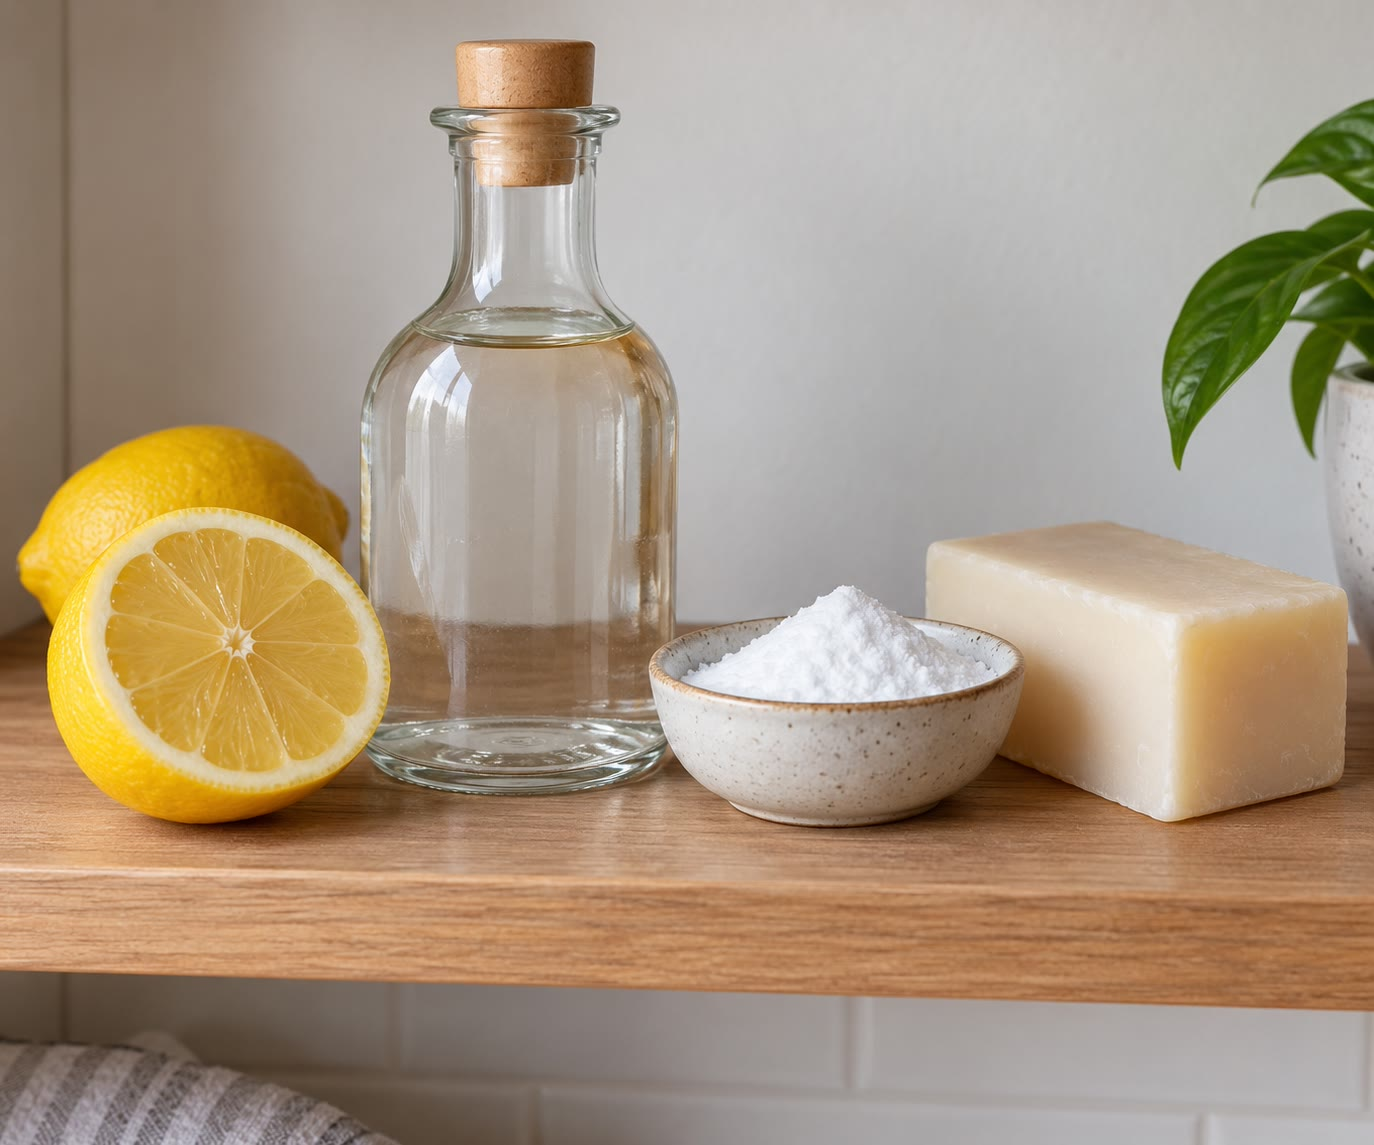
\includegraphics[width=0.55\linewidth]{images/book1/ai/g9-kitchen-shelf.jpg}

{\small الليمون والخل والصابون وصودا الخبز: أحماض وقواعد في
المطبخ.}
\end{omfigure}

\section{المحاليل الحمضية والقاعدية والمتعادلة}

\begin{definition}[المحاليل الحمضية والقاعدية والمتعادلة]\label{def:g9:acids-bases-ph:acidic}
كل \omterm{def:g6:solutions-and-solubility:solute}{محلول مائي} يحوي \omterm{def:g9:ions:ion}{أيونات} الهيدروجين \ce{H+(aq)} \omterm{def:g9:ions:ion}{وأيونات} الهيدروكسيد
\ce{OH-(aq)}. ويكون \omterm{def:g2:mixing-and-dissolving:dissolve}{المحلول} \emph{محلولًا حمضيًا}\index{محلول حمضي}
إذا كان يحوي من \omterm{def:g9:ions:ion}{أيونات} \ce{H+} أكثر مما يحوي من \omterm{def:g9:ions:ion}{أيونات} \ce{OH-}،
و\emph{محلولًا قاعديًا}\index{محلول قاعدي} إذا كان يحوي من \omterm{def:g9:ions:ion}{أيونات}
\ce{OH-} أكثر مما يحوي من \omterm{def:g9:ions:ion}{أيونات} \ce{H+}، و\emph{محلولًا
متعادلًا}\index{محلول متعادل} إذا كان يحوي منهما العدد نفسه.
\end{definition}

\begin{example}[ثلاثة محاليل]\label{ex:g9:acids-bases-ph:three}
حمض الهيدروكلوريك \omterm{def:g9:acids-bases-ph:acidic}{محلول حمضي}: فهو يحوي \omterm{def:g9:ions:ion}{أيونات} \ce{H+(aq)}
و\ce{Cl-(aq)}، وقليلًا جدًا من \ce{OH-}. \omterm{def:g2:mixing-and-dissolving:dissolve}{ومحلول} هيدروكسيد الصوديوم
قاعدي: \ce{Na+(aq)} و\ce{OH-(aq)}، وقليل جدًا من \ce{H+}. أما الماء
النقي والماء المالح فمتعادلان.
\end{example}

\section{سلّم pH}

\begin{definition}[pH]\label{def:g9:acids-bases-ph:ph}
\emph{pH}\index{pH} \omterm{def:g6:solutions-and-solubility:solute}{المحلول المائي}، أو رقمه الهيدروجيني، عدد يقع عادة بين 0 و14،
يدل على مدى حمضيته أو قاعديته: عند \qty{25}{\celsius} يكون pH \omterm{def:g9:acids-bases-ph:acidic}{المحلول المتعادل} 7،
وpH \omterm{def:g9:acids-bases-ph:acidic}{المحلول الحمضي} أقل من 7، وpH \omterm{def:g9:acids-bases-ph:acidic}{المحلول القاعدي} أكبر من 7. وكلما كثرت
\omterm{def:g9:ions:ion}{أيونات} \ce{H+} في \omterm{def:g2:mixing-and-dissolving:dissolve}{المحلول} انخفضت قيمة pH.
\end{definition}

\begin{omfigure}
\begin{tikzpicture}[font=\small, x=0.95cm]
  \foreach \k in {0,...,13} {
    \pgfmathtruncatemacro\rr{2.2*max(0,100-14.3*\k)+30}
    \pgfmathtruncatemacro\gg{1.8*(\k<7 ? 30+10*\k : 100-8*(\k-7))+40}
    \pgfmathtruncatemacro\bb{2.2*max(0,14.3*(\k-6))+30}
    \definecolor{phc}{RGB}{\rr,\gg,\bb}
    \fill[phc] (\k,0) rectangle ++(1,0.6);
  }
  \foreach \k in {0,...,14} \node[anchor=north, font=\footnotesize] at (\k,-0.02) {\k};
  \draw[black!60] (0,0) rectangle (14,0.6);
  \node[anchor=south] at (3.5,0.65) {حمضي};
  \node[anchor=south] at (7,0.65) {متعادل};
  \node[anchor=south] at (10.5,0.65) {قاعدي};
  % ledger: ph:HCl-1M, ph:gastric, ph:lime, ph:wine, ph:coffee, ph:pure-water, ph:seawater, ph:milk-magnesia, ph:ammonia, ph:NaOH-1M
  \foreach \x/\lab/\lev/\anc in {0/{حمض\\ \foreignlanguage{arabic}{الهيدروكلوريك \babelsublr{(1 M)}}}/1/north, 1.5/{العصارة\\ المعدية}/3/north east,
      2/{عصير\\ الليمون}/2/north west, 3.5/{النبيذ}/1/north, 5/{القهوة}/2/north, 7/{الماء\\ النقي}/3/north,
      8.1/{ماء\\ البحر}/1/north, 10.5/{حليب\\ المغنيسيا}/3/north, 12/{النشادر\\ المنزلي}/1/north,
      14/{هيدروكسيد الصوديوم\\ (1 M)}/2/north east} {
    \draw[black!55] (\x,-0.45) -- (\x,-0.45-0.8*\lev);
    \node[anchor=\anc, font=\footnotesize, align=center, inner sep=2pt] at (\x,-0.45-0.8*\lev) {\lab};
  }
\end{tikzpicture}

{\small سلّم \omterm{def:g9:acids-bases-ph:ph}{pH}، مع قيم \omterm{def:g9:acids-bases-ph:ph}{pH} لبعض المحاليل الشائعة.}
\end{omfigure}

\begin{definition}[ورق pH ومقياس pH]\label{def:g9:acids-bases-ph:ph-paper}
\emph{ورق pH}\index{ورق pH} شريط من الورق مشرّب \omterm{def:g6:pure-substances-and-mixtures:mixture}{بخليط} من الصبغات يأخذ
لونًا مختلفًا عند كل \omterm{def:g9:acids-bases-ph:ph}{pH}؛ توضع عليه قطرة من \omterm{def:g2:mixing-and-dissolving:dissolve}{المحلول} ويُقارن لونه بسلّم ألوان
مطبوع على العلبة. أما \emph{مقياس pH}\index{مقياس pH} فيقيس \omterm{def:g9:acids-bases-ph:ph}{pH} بمسبار
زجاجي يُغمس في \omterm{def:g2:mixing-and-dissolving:dissolve}{المحلول} ويعرضه عددًا، بمنزلة عشرية أو
منزلتين.
\end{definition}

\begin{method}[قياس pH بورق pH]\label{met:g9:acids-bases-ph:paper}
\begin{enumerate}
  \item ضع شريطًا قصيرًا من \omterm{def:g9:acids-bases-ph:ph-paper}{ورق pH} في صحن نظيف جاف.
  \item المس الشريط بقطرة من \omterm{def:g2:mixing-and-dissolving:dissolve}{المحلول} بواسطة ساق زجاجية نظيفة (ولا تغمس
        الشريط في القارورة أبدًا).
  \item قارن اللون فورًا بسلّم الألوان، واقرأ قيمة \omterm{def:g9:acids-bases-ph:ph}{pH}، وعادة إلى أقرب عدد
        صحيح.
\end{enumerate}
\end{method}

\begin{omfigure}
\begin{tikzpicture}[font=\small, scale=1.2]
  \pic[transform shape] at (0,0) {stirrer};
  \pic[transform shape] at (0,0.05) {beaker={0.55}{omWater!80}};
  \pic[transform shape] at (0.25,0.35) {probe};
  \pic[transform shape] at (2.6,3.4) {meter={pH}};
  \draw[black!70, line width=0.6pt] (0.25,3.45) .. controls (0.3,4.3) and (2.2,4.4)
    .. (2.2,2.95);
  \draw[<-, omProp, thick] (0.4,1.0) -- (2.0,1.3) node[right, text=black] {مسبار زجاجي};
  \draw[<-, omProp, thick] (3.35,3.4) -- (4.0,3.4) node[right, text=black] {\foreignlanguage{arabic}{مقياس \babelsublr{pH}}};
  \draw[<-, omProp, thick] (-0.6,0.6) -- (-1.6,0.9) node[left, text=black] {المحلول};
\end{tikzpicture}

{\small قياس \omterm{def:g9:acids-bases-ph:ph}{pH} \omterm{def:g9:acids-bases-ph:ph-paper}{بمقياس pH}: يُغمس المسبار الزجاجي في \omterm{def:g2:mixing-and-dissolving:dissolve}{المحلول}، الذي يُحرَّك
برفق.}
\end{omfigure}

\section{تخفيف حمض}

\begin{proposition}[التخفيف يقرّب pH من 7]\label{prop:g9:acids-bases-ph:dilution}
إضافة الماء إلى \omterm{def:g9:acids-bases-ph:acidic}{محلول حمضي} تنشر \omterm{def:g9:ions:ion}{أيونات} \ce{H+} فيه في حجم أكبر: فيرتفع
\omterm{def:g9:acids-bases-ph:ph}{pH} نحو 7، لكنه لا يتجاوزه أبدًا. ولحمض مثل حمض الهيدروكلوريك، يرفع
التخفيف عشر مرات قيمة \omterm{def:g9:acids-bases-ph:ph}{pH} بنحو وحدة واحدة: حجم واحد من حمض \omterm{def:g9:acids-bases-ph:ph}{pH} له 2 مع تسعة
أحجام من الماء يعطي \omterm{def:g2:mixing-and-dissolving:dissolve}{محلولًا} \omterm{def:g9:acids-bases-ph:ph}{pH} له 3. وتخفيف \omterm{def:g9:acids-bases-ph:acidic}{محلول قاعدي} يخفض \omterm{def:g9:acids-bases-ph:ph}{pH} بالمثل
نحو 7.
\end{proposition}

\begin{omfigure}
\begin{tikzpicture}[font=\small, scale=1.05]
  \foreach \k/\ph/\cc in {0/2/red!38!omWater,1/3/red!24!omWater,2/4/red!12!omWater} {
    \pic[transform shape] at (\k*4.4,0) {beaker={0.55}{\cc}};
    \node[anchor=north, align=center] at (\k*4.4,-0.15) {pH \ph};
  }
  \foreach \k in {0,1} \draw[->, thick, omProp] (\k*4.4+1.1,1.0) -- (\k*4.4+3.3,1.0)
    node[midway, above, text=black, font=\footnotesize, align=center]
    {10 mL + 90 mL\\ من الماء};
\end{tikzpicture}

{\small تخفيف حمض عشر مرات، ثم عشر مرات من جديد: تمر قيمة \omterm{def:g9:acids-bases-ph:ph}{pH} من 2 إلى 3 إلى
4 (كل كأس عُشر \omterm{def:g2:mixing-and-dissolving:dissolve}{المحلول} السابق أُكمل بالماء).}
\end{omfigure}

\begin{inthelab}[تخفيف حمض]
لتخفيف حمض يصب المعلم الحمض دائمًا ببطء في الماء، لا الماء في الحمض أبدًا:
\omterm{def:g2:mixing-and-dissolving:mix}{فالخلط} يطلق حرارة، والماء الذي يُصب على حمض مركّز قد يغلي في الحال فيقذف
الحمض خارج الوعاء.
\end{inthelab}

\section{أحماض وقواعد يومية}

\begin{proposition}[الأحماض والقواعد من حولنا]\label{prop:g9:acids-bases-ph:everyday}
حمضية: عصير الليمون الأصفر والأخضر، والخل، والنبيذ، والمشروبات الغازية،
والقهوة، والعصارة المعدية في المعدة. قاعدية: ماء البحر (قليلًا)، وصودا
الخبز المذابة في الماء، والصابون، وحليب المغنيسيا (دواء لحموضة المعدة)،
والنشادر المنزلي، وماء الجافيل، ومنظّف المجاري (بشدة كبيرة).
\end{proposition}

\begin{example}[pH المحيط]\label{ex:g9:acids-bases-ph:ocean}
% ledger: ph:seawater, ph:ocean-drop
متوسط \omterm{def:g9:acids-bases-ph:ph}{pH} المحيط نحو 8.1: قاعدي قليلًا. ومنذ بداية العصر الصناعي خفض
ثنائي أكسيد الكربون الذائب من \omterm{def:g4:air-a-mixture-of-gases:air}{الهواء} \omterm{def:g9:acids-bases-ph:ph}{pH} المياه السطحية بنحو 0.1: فالمحيطات
تصير شيئًا فشيئًا أقل قاعدية، وهذا يضر بالمحاريات
والمرجان.
\end{example}

\begin{omfigure}
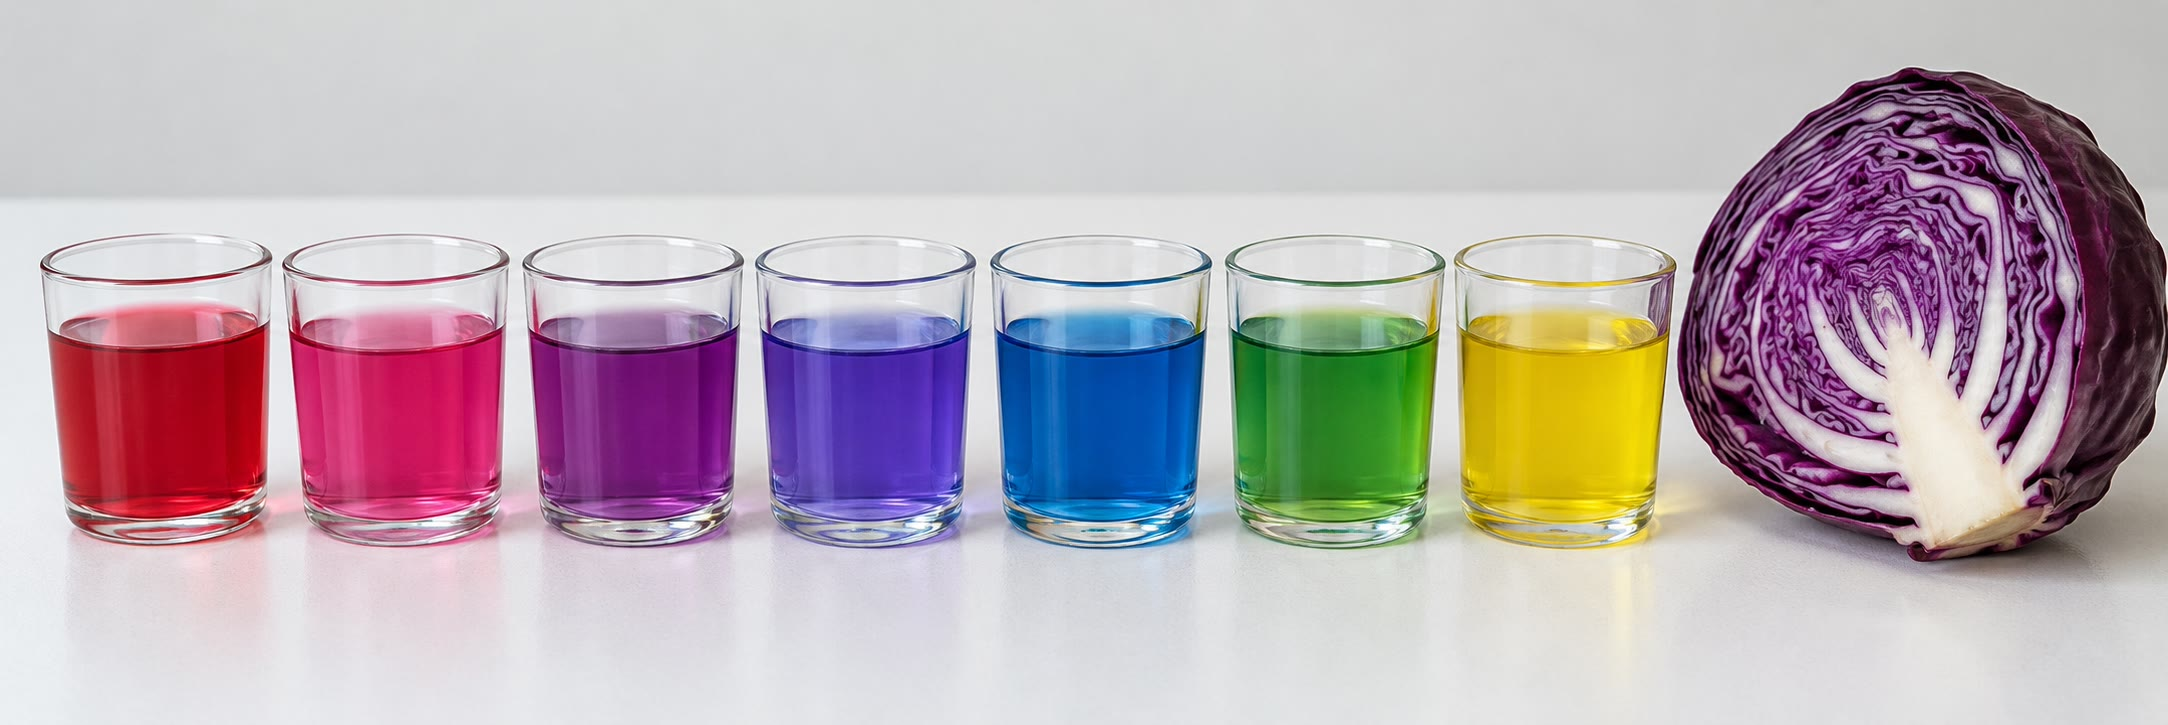
\includegraphics[width=0.55\linewidth]{images/book1/ai/g9-red-cabbage.jpg}

{\small عصير الملفوف الأحمر، الذي يحضّره المعلم، يتغير لونه مع \omterm{def:g9:acids-bases-ph:ph}{pH}: أحمر
في الأحماض، وبنفسجي قرب التعادل، ثم أزرق فأخضر فأصفر في المحاليل التي
تزداد قاعديتها.}
\end{omfigure}

\section{السلامة مع المنتجات الأكّالة}

\begin{safety}{\ghs[0.85cm]{GHS05}\ghs[0.85cm]{GHS07}}
% ledger: ghs:HCl, ghs:NaOH
حمض الهيدروكلوريك المركّز وهيدروكسيد الصوديوم (قاعدة منظّفات المجاري) يحملان
رمز التآكل GHS05: فهما يسببان حروقًا شديدة للجلد والعينين ويهاجمان
الفلزات. GHS07: مهيّج. نظارات واقية وقفازات؛ ويُشطف أي رذاذ فورًا بكثير من
الماء.
\end{safety}

\begin{remark}[لا تخلط منتجات التنظيف أبدًا]\label{rem:g9:acids-bases-ph:mix}
المنتجات الحمضية والقاعدية تتفاعل معًا، بعنف أحيانًا، وبعض الخلائط يطلق
غازات سامة: فماء الجافيل المخلوط بمزيل كلس حمضي يطلق الكلور. ولا تُخلط
منتجات التنظيف أبدًا.
\end{remark}

\section{تمارين}

\begin{exercise}[$\star$]\label{exo:g9:acids-bases-ph:1}
حمضي أم قاعدي أم متعادل؟ \omterm{def:g2:mixing-and-dissolving:dissolve}{محلول} \omterm{def:g9:acids-bases-ph:ph}{pH} له 3، وآخر \omterm{def:g9:acids-bases-ph:ph}{pH} له 7، وثالث
\omterm{def:g9:acids-bases-ph:ph}{pH} له 11.
\end{exercise}

\begin{exercise}[$\star$]\label{exo:g9:acids-bases-ph:2}
أي \omterm{def:g9:ions:ion}{الأيونات} أكثر عددًا في \omterm{def:g9:acids-bases-ph:acidic}{المحلول الحمضي}؟ وفي \omterm{def:g9:acids-bases-ph:acidic}{المحلول القاعدي}؟
\end{exercise}

\begin{exercise}[$\star$]\label{exo:g9:acids-bases-ph:3}
مستعينًا بسلّم \omterm{def:g9:acids-bases-ph:ph}{pH} في هذا الفصل، رتّب من الأشد حمضية إلى الأشد قاعدية:
القهوة، وماء البحر، وعصير الليمون، والنشادر المنزلي، والماء
النقي.
\end{exercise}

\begin{exercise}[$\star$]\label{exo:g9:acids-bases-ph:4}
صف كيف تقيس \omterm{def:g9:acids-bases-ph:ph}{pH} \omterm{def:g2:mixing-and-dissolving:dissolve}{محلول} \omterm{def:g9:acids-bases-ph:ph-paper}{بورق pH}.
\end{exercise}

\begin{exercise}[$\star\star$]\label{exo:g9:acids-bases-ph:5}
\omterm{def:g2:mixing-and-dissolving:dissolve}{محلول} \omterm{def:g9:acids-bases-ph:ph}{pH} له 4 يُخفَّف عشر مرات بالماء. ما قيمة \omterm{def:g9:acids-bases-ph:ph}{pH} الجديدة تقريبًا؟
وإذا خُفّف مئة مرة؟
\end{exercise}

\begin{exercise}[$\star\star$]\label{exo:g9:acids-bases-ph:6}
هل يمكن أن يصير \omterm{def:g9:acids-bases-ph:acidic}{محلول حمضي} قاعديًا بإضافة الماء؟ علّل.
\end{exercise}

\begin{exercise}[$\star\star$]\label{exo:g9:acids-bases-ph:7}
لماذا يجب أن يُصب الحمض في الماء، لا العكس؟
\end{exercise}

\begin{exercise}[$\star\star$]\label{exo:g9:acids-bases-ph:8}
قارورة تحمل رمز الخطر GHS05. ماذا يعني؟ اذكر
احتياطين.
\end{exercise}

\begin{exercise}[$\star\star$]\label{exo:g9:acids-bases-ph:9}
كم تخفيفًا بعشرة أضعاف يلزم لنقل حمض من \omterm{def:g9:acids-bases-ph:ph}{pH} 1 إلى
\omterm{def:g9:acids-bases-ph:ph}{pH} 4؟ وما التخفيف الكلي؟
\end{exercise}

\begin{exercise}[$\star\star$]\label{exo:g9:acids-bases-ph:10}
يؤخذ حليب المغنيسيا لحموضة المعدة. استعن بسلّم \omterm{def:g9:acids-bases-ph:ph}{pH}
لتشرح لماذا.
\end{exercise}

\begin{exercise}[$\star\star\star$]\label{exo:g9:acids-bases-ph:11}
انخفض \omterm{def:g9:acids-bases-ph:ph}{pH} المحيط بنحو 0.1 منذ العصر الصناعي. هل المحيط حمضي اليوم؟ وفي أي
اتجاه يسير، ولماذا؟
\end{exercise}

\begin{exercise}[$\star\star\star$]\label{exo:g9:acids-bases-ph:12}
يقيس تلميذ \omterm{def:g9:acids-bases-ph:ph}{pH} الخل نفسه \omterm{def:g9:acids-bases-ph:ph-paper}{بورق pH} (3) وبمقياس \omterm{def:g9:acids-bases-ph:ph}{pH} (2.6). اشرح لماذا تختلف
النتيجتان، وأيهما أدق.
\end{exercise}

\section{مسألة: انسكاب الحمض}

\begin{problem}[{مسألة نهاية الأسبوع --- لتر من الحمض انسكب في مغسلة
المختبر، ولماذا لا يكون التخفيف هو الحل}]
\label{pb:g9:acids-bases-ph:1}
تنكسر في مغسلة المختبر قارورة فيها \qty{1}{L} من حمض الهيدروكلوريك المخفف،
\omterm{def:g9:acids-bases-ph:ph}{pH} له 2. ولا يجوز أن يتلقى المجرى أي \omterm{def:g2:mixing-and-dissolving:dissolve}{محلول} \omterm{def:g9:acids-bases-ph:ph}{pH} له أقل من 5. خذ قاعدة هذا
الفصل: لهذا الحمض، كل تخفيف بعشرة أضعاف يرفع \omterm{def:g9:acids-bases-ph:ph}{pH} وحدة
واحدة.

\medskip
\noindent\textbf{الجزء الأول --- الحمض.}
\begin{enumerate}
  \item هل \omterm{def:g9:acids-bases-ph:acidic}{المحلول حمضي} أم متعادل أم قاعدي؟ وأي \omterm{def:g9:ions:ion}{الأيونات} أكثر فيه؟
  \item أي رمز خطر يجب أن تحمل القارورة، ولماذا؟
  \item يقيس المعلم \omterm{def:g9:acids-bases-ph:ph}{pH} \omterm{def:g9:acids-bases-ph:ph-paper}{بمقياس pH} بدلًا من \omterm{def:g9:acids-bases-ph:ph-paper}{ورق pH}.
        أعطِ ميزة واحدة.
  \item كم مرة تزيد \omterm{def:g9:ions:ion}{أيونات} \ce{H+} في لتر \omterm{def:g9:acids-bases-ph:ph}{pH} له 2 على ما في لتر \omterm{def:g9:acids-bases-ph:ph}{pH} له 3
        من الحمض نفسه؟
\end{enumerate}

\medskip
\noindent\textbf{الجزء الثاني --- التخفيف.}
\begin{enumerate}[resume]
  \item ما حجم \omterm{def:g2:mixing-and-dissolving:dissolve}{المحلول} الذي نحصل عليه بتخفيف لتر الحمض عشر مرات؟ وما
        قيمة \omterm{def:g9:acids-bases-ph:ph}{pH} له؟
  \item كم تخفيفًا بعشرة أضعاف يلزم لبلوغ \omterm{def:g9:acids-bases-ph:ph}{pH} 5؟
  \item ما الحجم الكلي \omterm{def:g2:mixing-and-dissolving:dissolve}{للمحلول} الذي ينتج عن ذلك؟
  \item هل يمكن لأي مقدار من الماء أن يجعل \omterm{def:g2:mixing-and-dissolving:dissolve}{المحلول} قاعديًا؟ علّل.
\end{enumerate}

\medskip
\noindent\textbf{الجزء الثالث --- طريقة أفضل.}
يضيف المعلم بدلًا من ذلك، شيئًا فشيئًا، \omterm{def:g2:mixing-and-dissolving:dissolve}{محلول} قاعدة حتى يبيّن \omterm{def:g9:acids-bases-ph:ph-paper}{ورق pH} القيمة
7: فتتفاعل \omterm{def:g9:ions:ion}{أيونات} \ce{H+} في الحمض مع \omterm{def:g9:ions:ion}{أيونات} \ce{OH-}
في القاعدة.
\begin{enumerate}[resume]
  \item اكتب معادلة التفاعل بين \omterm{def:g9:ions:ion}{أيونات} \ce{H+} \omterm{def:g9:ions:ion}{وأيونات}
        \ce{OH-}.
  \item لماذا يكون هذا أفضل من التخفيف؟
  \item سمِّ منتجًا قاعديًا يوميًا يمكن استعماله في المطبخ لتنظيف انسكاب صغير
        من الخل.
  \item احسب حجم الماء الذي كان يلزم إضافته إلى لتر الحمض لبلوغ
        \omterm{def:g9:acids-bases-ph:ph}{pH} 5.
\end{enumerate}
\end{problem}
